\documentclass[french]{report}

\usepackage{hyperref}
\usepackage{graphicx}

% TOC
\setcounter{secnumdepth}{-1}

% Layout
\setlength{\parindent}{0em}
\setlength{\parskip}{1em}
\linespread{1.6}

% Language
\usepackage[utf8]{inputenc}
\usepackage[frenchb]{babel}
\usepackage[autostyle=true,french=guillemets]{csquotes}

% Code listings and figures
\usepackage{listings}
\usepackage{xcolor}
\usepackage{float}
\usepackage{subfig}
\usepackage[scaled=0.85]{beramono}
\usepackage[lighttt]{lmodern}
\floatstyle{boxed} 
\restylefloat{figure}
\captionsetup{belowskip=12pt,aboveskip=4pt}

\lstset{
	basicstyle={\linespread{1}\ttfamily},
	extendedchars=true,
	framesep=10pt,
	xleftmargin=25pt,
	xrightmargin=10pt,
	literate={á}{{\'a}}1 {ã}{{\~a}}1 {é}{{\'e}}1 {É}{{\'E}}1,
	numbers=left,
	numbersep=10pt,
	escapeinside={(*@}{@*)}
}

% Title Page
\title{Eiffel et OCaml---deux langages, deux approches pour obtenir la qualité des logiciels}
\author{Ross Gardiner}


\begin{document}
\maketitle

\tableofcontents

\chapter{Introduction}

De nos jours, les logiciels sont partout : portables, avions, lave-vaisselles, lampes. Pour citer Marc Andreessen, \enquote{les logiciels mangent le monde}. Malheureusement, ces logiciels sont souvent bogués, m\^{e}me dangereux.

Depuis de nombreuses années, l’industrie du logiciel essaye de trouver des méthodes pour améliorer la qualité de son logiciel. Plusieurs éminents informaticiens français ont développé des nouveaux langages à cette fin. Dans ce projet, je décrirai deux langages de programmation : Eiffel et OCaml. Les deux tentent d’assurer la sécurité contre les bogues et les comportements inattendus, mais ils ont des approches assez différentes. Je vais examiner et comparer leurs fonctionnements et leurs caractéristiques.

Bien qu'OCaml---datant de 1996---soit plus récent qu'Eiffel---de 1986---ses origines sont plutôt plus anciennes.  OCaml dérive de ML, développé à Édimbourg en 1973. OCaml lui-m\^{e}me a débuté à l’INRIA, un institut de recherche français. Eiffel a été créé par Bertrand Meyer, un informaticien français qui est actuellement professeur de génie logiciel à l’ETH Zurich.

Eiffel est un langage \enquote{orienté objet}, ce qui signifie qu'il modèle le monde comme une collection d’objets. Chaque objet peut effectuer des actions (\enquote{commandes}), et chaque objet a des propriétés (\enquote{requêtes}).

Par contre, OCaml est un langage multi-paradigme---mais, premièrement, c’est un langage fonctionnel. Dans un tel langage, les informations et les actions sont strictement séparées. Nous examinerons les conséquences de ces conceptions dans le reste du projet.

\chapter{Eiffel}

Eiffel a été conçu avec un seul objectif : améliorer la qualité de logiciel. La plupart de sa fonctionnalité est destinée à servir cet objectif.
 
\section{La conception par contrat}

La caractéristique la plus inhabituelle d'Eiffel est « la conception par contrat ». Très souvent, lorsque les informaticiens veulent prouver qu’un algorithme est correct, ils utilisent les \enquote{préconditions}, les \enquote{postconditions} et les \enquote{invariants}. Si on examine un fragment de code, une précondition est un fait qui doit être vraie juste avant l’exécution du code. De même, une postcondition doit être vraie juste après l’exécution. Un invariant doit être vrai en tout temps.

La plupart des langages n'encodent pas	ces concepts mathématiques, mais Eiffel l'incite. La Figure \ref{fig:pre-post-condition} montre un exemple. Nous définissons une classe qui représente un compte bancaire. C'est très simple. Premièrement, il y a un attribut \texttt{solde} qui stocke la somme d'argent qui est actuellement dans le compte. En outre, il y a une routine \texttt{dépose} qui prend en argument un montant d'argent pour ajouter au compte. Le bloc \texttt{require} contient une précondition: nous ne pouvons pas ajouter un montant négatif au compte. Le block \texttt{ensure} contient une postcondition: après avoir déposé un montant, le solde du compte doit être le solde initial plus la somme ajoutée.

\begin{figure}[h]
	\begin{lstlisting}[language=Eiffel]
class COMPTE_BANCAIRE

feature
  solde: INTEGER

  dépose (somme: INTEGER)
    require
      somme >= 0
    do
      solde := solde + somme
    ensure
      solde = old solde + somme
  end
end
	\end{lstlisting}
	
	\caption{Un exemple d'utiliser une précondition et une postcondition\protect\footnotemark}
	\label{fig:pre-post-condition}
\end{figure}

\footnotetext{Adapté de \url{https://archive.eiffel.com/doc/online/eiffel50/intro/language/invitation-07.html}}

\section{La séparation commande-requête}

Cet exemple montre aussi le principe de séparation commande-requête. \texttt{solde} est une requête---elle retourne le solde, mais elle ne peut pas changer l'état du compte. En revanche, \texttt{dépose} est une commande. Elle ne donne un résultat, mais elle changera l'état du compte. Ce principe rassure le programmeur que l'extraction du solde ne causera pas des effets secondaires inattendus.

\begin{figure}[h]
	\begin{lstlisting}[language=Eiffel]
class APPLICATION

feature
  principal
    local
      compte: COMPTE_BANCAIRE 	(*@\label{line:reference-declaration}@*)
    do
      print (compte.somme)		(*@\label{line:null-deref}@*)
    end
end
	\end{lstlisting}
	
	\caption{Un exemple d'un déréférencement d'un pointeur nul}
	\label{fig:null-deref-condition}
\end{figure}

\begin{figure}[h]
	\begin{lstlisting}[language=Eiffel]
class APPLICATION
	
feature
  principal
    local
      compte: COMPTE_BANCAIRE
    do
      create compte 		(*@\label{line:object-creation}@*)
      print (compte.somme) 	
    end
end
	\end{lstlisting}
	
	\caption{Un exemple d'une initialisation correcte d'un pointeur}
	\label{fig:nonnull-deref-condition}
\end{figure}

\section{La sécurité contre le déréférencement de pointeurs nuls}

Eiffel empêche aussi un problème rencontré souvent dans d'autres langages---le déréférencement de pointeurs nuls. Ceci se produit lorsqu'on crée une référence mais ne l'attache jamais à un objet. Comparez les figures \ref{fig:null-deref-condition} et \ref{fig:nonnull-deref-condition}. Figure \ref{fig:null-deref-condition} montre une situation courante dans les autres langages. Une référence \texttt{compte} est déclarée par la ligne \ref{line:reference-declaration}, mais aucun objet réel est créé. Quand l'instruction \texttt{print (compte.somme)} (ligne \ref{line:null-deref}) est exécutée, le logiciel plantera. Figure \ref{fig:nonnull-deref-condition} est une version correcte : \texttt{compte} est initialisé par l'instruction \texttt{create compte} (ligne \ref{line:object-creation}). Eiffel détecte automatiquement la version incorrecte, qui empêche beaucoup de plantages.

\section{Réutilisabilité et extensibilité}

Deux des grands principes d'Eiffel sont réutilisabilité et extensibilité. Ces mots résume l'idée que les logiciels doivent---autant que possible---être réutilisés ou modifiés plutôt que développés à partir de zéro. Le but est---dans tout nouveau système---de maximiser la quantité du code qui a déjà fait ses preuves.

Eiffel offre toutes les méthodes normales pour permettre la réutilisabilité et l'extensibilité---par exemple l'héritage, les bibliothèques communes et les classes génériques. Cependant, Eiffel a une approche intéressant pour faire l'héritage multiple.

\begin{figure}[h]
	\centering
	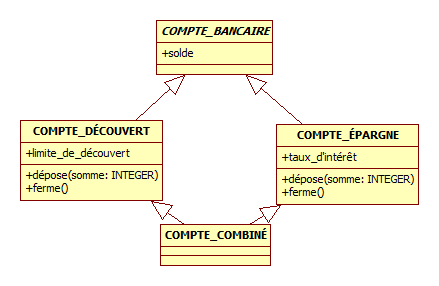
\includegraphics[width=0.7\linewidth]{multiple_inheritance}
	\caption{Un exemple du héritage multiple}
	\label{fig:multiple-inheritance}
\end{figure}

Dans la figure \ref{fig:multiple-inheritance} il y a un exemple du héritage multiple. Nous définissons un simple compte bancaire avec juste un solde. Les types plus précis de compte sont un compte avec un solde à découvert, un compte d'épargne et un compte qui combine les deux. Les deux classes \texttt{COMPTE\_DÉCOUVERT} et \texttt{COMPTE\_ÉPARGNE} définissent les routines supplémentaires \texttt{dépose(somme: INTEGER)} et \texttt{ferme}. Que devrait faire le \texttt{COMPTE\_COMBINÉ} quand ces routines s'appellent? Eiffel propose quelques solutions.


\begin{figure}[h]
	\begin{lstlisting}[language=Eiffel]
class COMPTE_COMBINÉ
  inherit COMPTE_DÉCOUVERT
    redefine	(*@\label{line:redefine}@*)
      dépose
    rename		(*@\label{line:rename}@*)
      ferme as ferme_découvert
  end
  
  inherit COMPTE_ÉPARGNE
    redefine
      dépose
    rename
      ferme as ferme_épargne
  end
  
  feature
    dépose (somme: INTEGER)
      do
        ...
      end
end
	\end{lstlisting}
	
	\caption{Un exemple d'héritage multiple avec Eiffel}
	\label{fig:multiple-inheritance-code}
\end{figure}

La figure \ref{fig:multiple-inheritance-code} montre deux des outils de gestion d'héritage multiple. \texttt{redefine dépose} (ligne \ref{line:redefine}) signifie que les mises en oeuvre de \texttt{dépose} (par \texttt{COMPTE\_DÉCOUVERT} et \texttt{COMPTE\_ÉPARGNE}) sont à être ignorées et remplacées par une nouvelle définition dans \texttt{COMPTE\_COMBINÉ}.

Par ailleurs, nous pouvons aussi renommer les fonctionnalités : ici, le \texttt{ferme} de \texttt{COMPTE\_DÉCOUVERT} devient \texttt{ferme\_découvert} (ligne \ref{line:rename}). Quoiqu'on fasse, Eiffel garantit que les préconditions, les postconditions et les invariants sont observés.

Ce système permet la réutilisation de plusieurs classes dans une seule classe dérivée.

\chapter{OCaml}

Comparé à Eiffel, OCaml n'est pas aussi concentré sur la prévention des erreurs. Malgré cela, une partie significative de sa fonctionnalité est utile pour écrire du code stable.

\section{La programmation \enquote{fonctionnelle} et l'immutabilité par défaut}

OCaml incitera fortement un style de la programmation \enquote{fonctionnelle}. Le style traditionnel de la programmation est \enquote{impératif}. Dans celle-là, on évite de causer des effets secondaires---alors que dans celle-ci les effets secondaires sont la norme. Un effet secondaire clé est la modification des données (la \enquote{mutation}).

\begin{figure}[h]
	\centering
	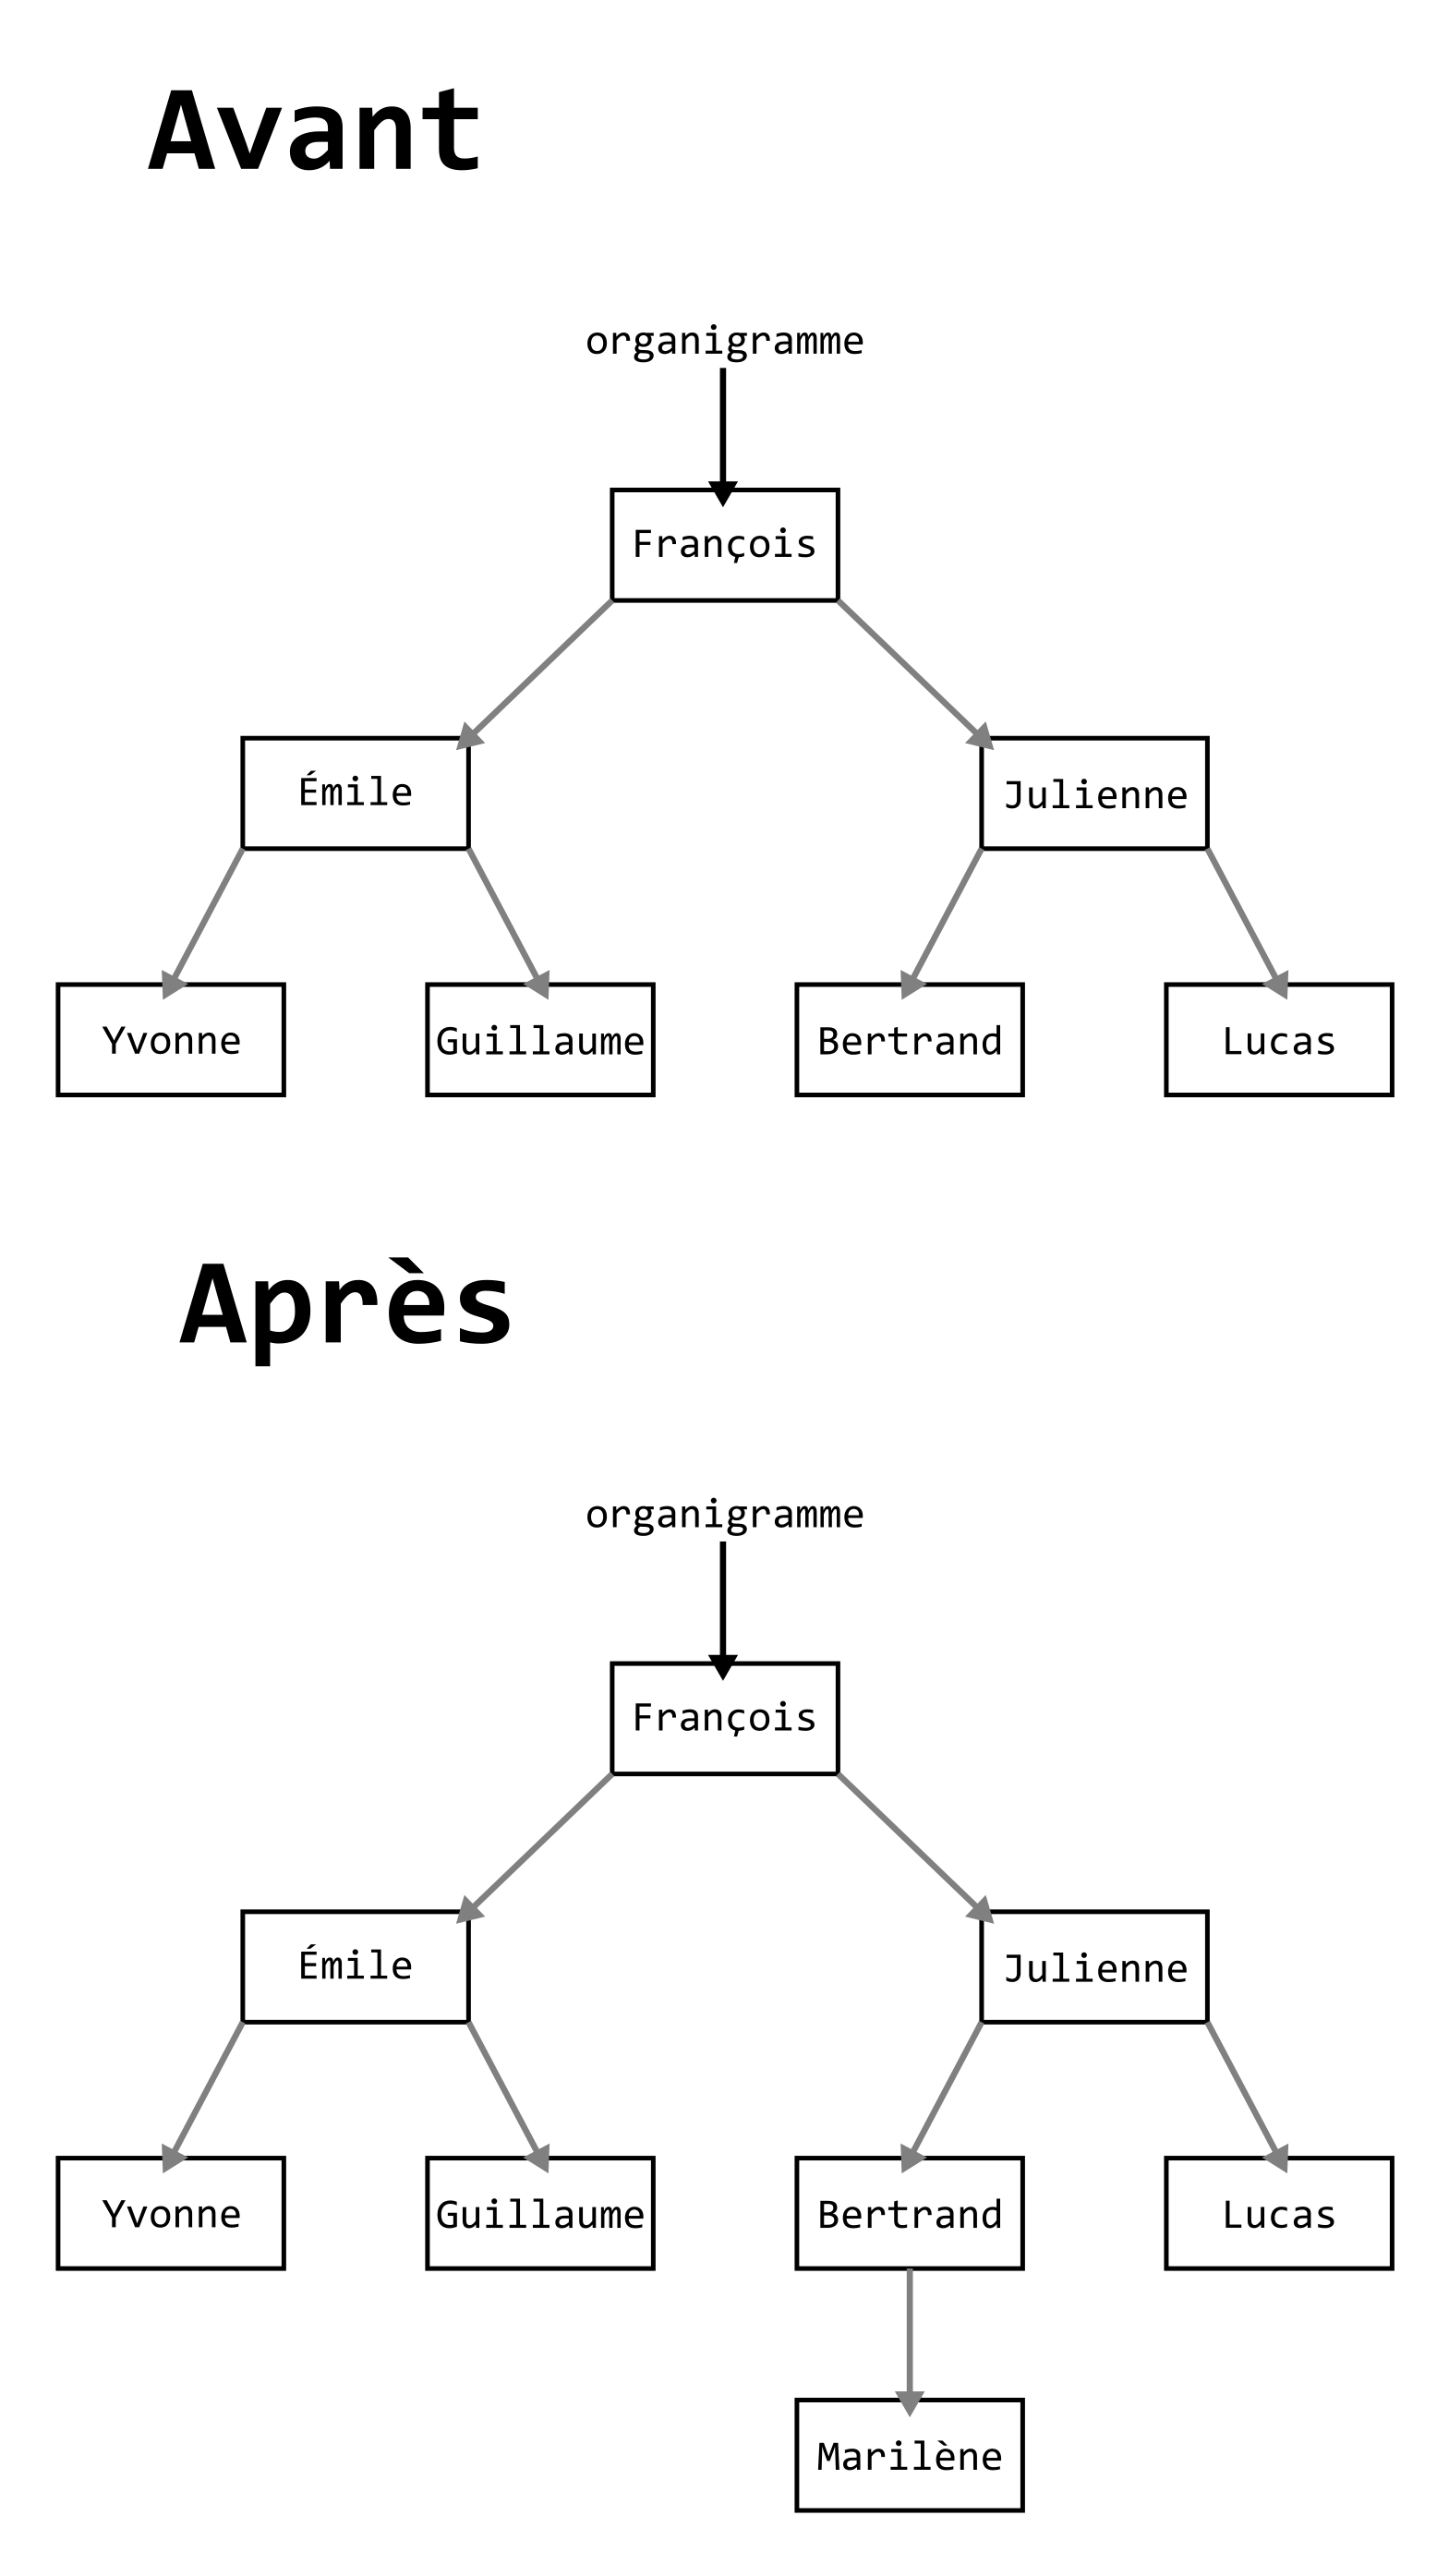
\includegraphics[width=0.7\linewidth]{mutable_tree}
	\caption{Un exemple d'une structure des données mutable}
	\label{fig:mutable-tree}
\end{figure}

\begin{figure}[h]
	\centering
	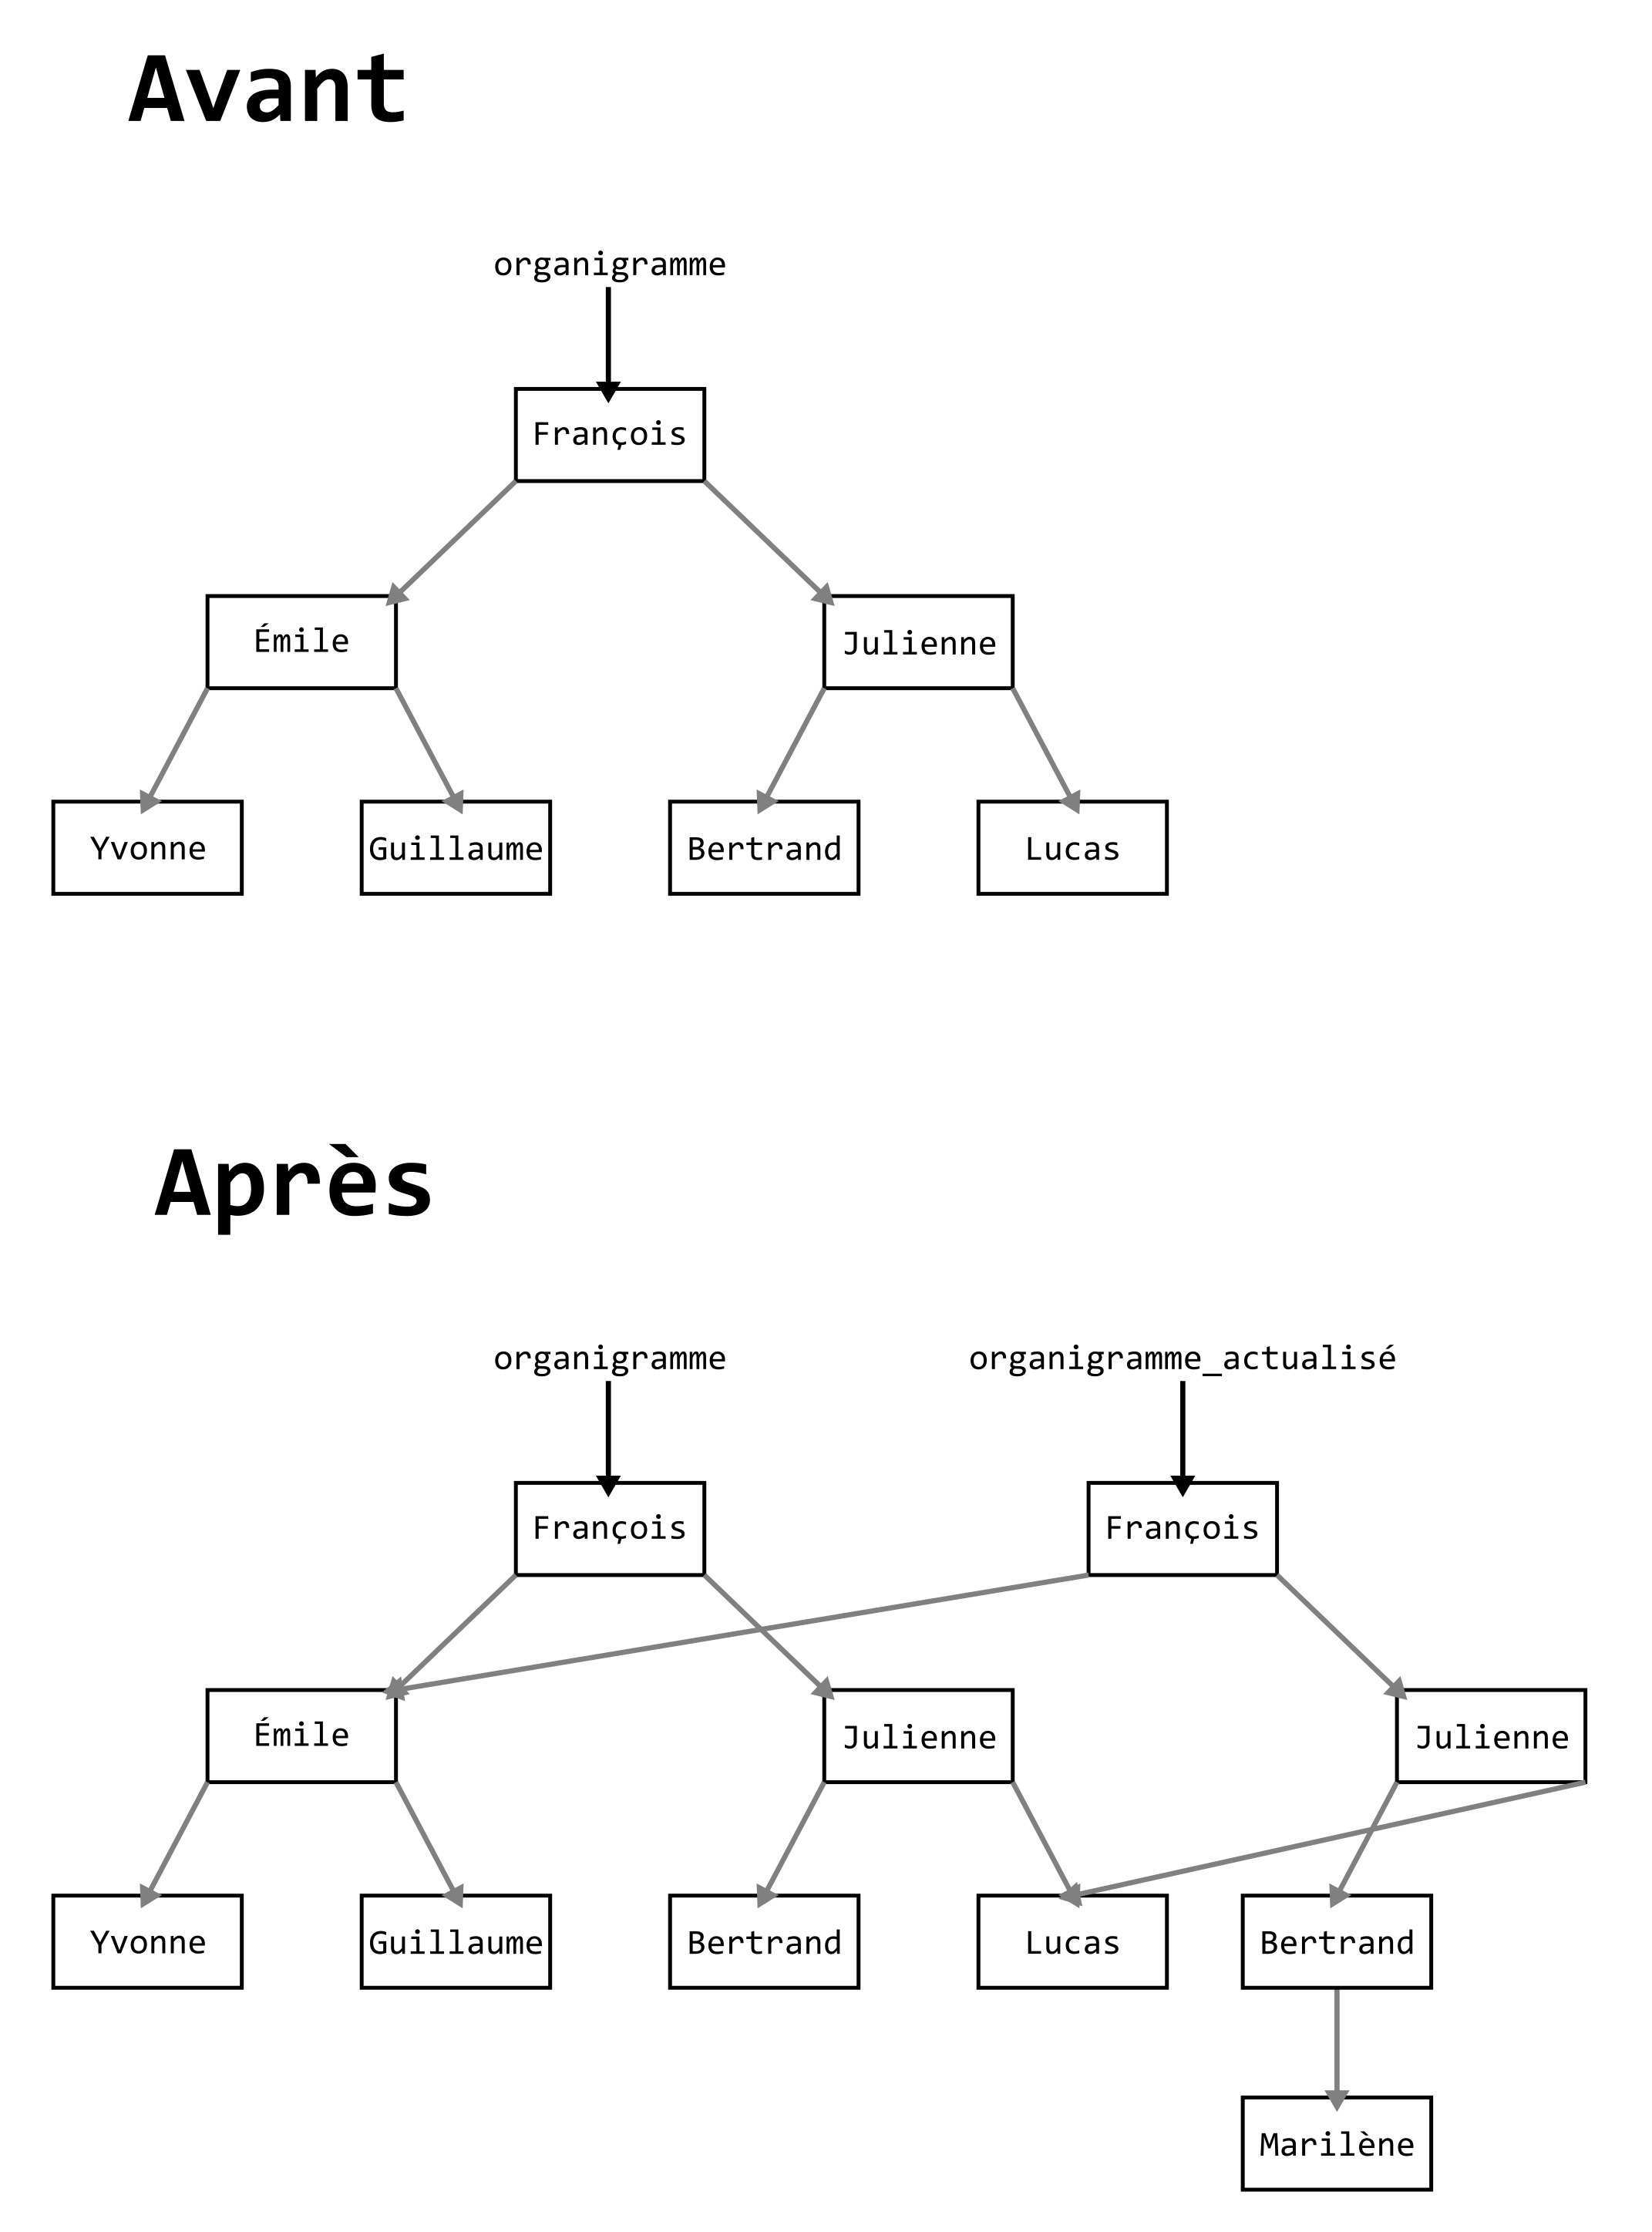
\includegraphics[width=0.7\linewidth]{immutable_tree}
	\caption{Un exemple d'une structure des données immuable}
	\label{fig:immutable-tree}
\end{figure}

La figure \ref{fig:mutable-tree} montre un organigramme qui est mis à jour dans un langage impératif. Après l'opération, la référence originale (\texttt{organigramme}) pointe à la même structure d'arbre, mais la structure a été modifiée. N'importe quel code qui utilise cet organigramme doit savoir que d'autres parties de code peuvent le modifier.

La figure \ref{fig:immutable-tree} montre un organigramme dans un langage fonctionnel. L'opération ne modifie pas l'arbre original, mais elle plutôt crée une nouvelle référence et elle fabrique une nouvelle copie seulement de la partie d'arbre qui change. Les deux versions du organigramme peuvent bien coexister. Le code qui utilise la référence \texttt{organigramme} peut supposer que les données ne changent jamais.

Nous reconnaissons depuis peu que les structures des données immuables sont souvent préférable. Elles facilitent de raisonner sur le comportement d'un programme parce qu'on n'a pas à se soucier de la possibilité que les données peuvent être changées de manière imprévue.

\begin{figure}[h]
	\begin{lstlisting}[language=Caml]
let construis_message verbeux message = 
  if verbeux then message else ""
	\end{lstlisting}
	
	\caption{Un exemple de l'inférence de types en OCaml\protect\footnotemark}
	\label{fig:type-inference-code}
\end{figure}

\footnotetext{Adapté de \url{https://www.cis.upenn.edu/~sweirich/icfp-plmw15/slides/pottier.pdf}}

\begin{figure}[h]
	\begin{lstlisting}[language=Eiffel]
construis_message (verbeux: BOOLEAN; 
                   message: STRING): STRING
  do
    if verbeux then
      Result := message
    else
      Result := ""
  end
end
	\end{lstlisting}
	\caption{Une requête qui équivaut à la Figure \ref{fig:type-inference-code}}
	\label{fig:without-type-inference-code}
\end{figure}

\section{L'inférence de types et la concision}

OCaml et Eiffel sont langages à typage statique. Cela signifie qu'on sait le type de chaque valeur dans un programme---par exemple: un nombre entier, un nombre réel, une chaîne de caractères, un organigramme. Cependant, il y a une différence clé. En Eiffel, on doit indiquer le type d'un valeur très explicitement.

La figure \ref{fig:type-inference-code} montre une fonction en OCaml qui construit un message. La fonction prend deux arguments: \texttt{verbeux}, qui indique si le résultat devrait être verbeux, et \texttt{message}, qui est le message verbeux. Le message non-verbeux est une chaîne vide. On ne précise jamais les types exacts de \texttt{verbeux} ou \texttt{message}: OCaml les calcule automatiquement. \texttt{verbeux} doit être booléen, également \texttt{message} doit être une chaîne de caractères.

Comparez avec Eiffel (la Figure \ref{fig:without-type-inference-code}): on doit écrire \texttt{: BOOLEAN} et \texttt{: STRING} pour indiquer les types. Le code est beaucoup plus long. La force d'OCaml est qu'il permet aux programmeurs d'écrire des programmes concis et compréhensible. Ces qualités rendent la maintenance plus facile.

\section{L'application partielle et la composition de fonctions}

Un autre aspect intéressant d'OCaml est l'application partielle de fonctions. Ceci utilise la curryfication, qui transforme une fonction à plusieurs arguments à une série de fonctions à un argument. Par exemple, considérez la fonction \texttt{add x y = x + y}, qui prend deux nombres entiers et renvoie la somme. Évidemment, \texttt{add 2 3} renvoie \texttt{5}.

On peut considérer cette fonction comme \texttt{(entier, entier) -> entier}: elle prend deux entiers et renvoie un entier. En fait, OCaml considère la fonction comme \texttt{entier -> (entier -> entier)}: une fonction qui prend un entier et renvoie une deuxième fonction, qui prend un entier et renvoie un entier. 

On peut appliquer la fonction partiellement ainsi: \texttt{add6 = (add 6)}. Ceci rend \texttt{add2} comme une fonction \texttt{entier -> entier}. Elle prend un entier et le renvoie plus six. Par exemple, \texttt{add6 3} renvoie \texttt{9}.

L'application partielle, entre autres outils, est un mécanisme puissant de combinaison de fonctions. Cela permet la réutilisation simple et fiable du code, un facteur important pour la qualité.

\end{document}          

% Points to compare:
% - command-request separation vs pure functions/immutability/referential transparency
%   bizarrely, OCaml provides less guarantees than Eiffel - but encourages better style
% - object-oriented vs functional - reliance on side effects means problems easier to model
%   in Eiffel but harder to reason about once written
% - reusability - composition vs inheritance
% - failings of both compared to other languages - Haskell, Idris, (Coq? - it's french),
%   compiler certification